\subsection{Optimizations for LPA}
\label{sec:lpa}

We use a parallel implementation of LPA and experiment with different optimizations and parameter settings. We use the \textit{asynchronous} version of LPA, wherein threads operate independently on distinct regions of the graph. This facilitates quicker convergence, but may introduce greater variability in the final result. Further, we observe that parallel LPA obtains communities of higher quality than its sequential implementation, possibly due to randomization. We allocate a separate hashtable per thread to keep track of the total weight of each unique label linked to a vertex.

Our optimizations include using OpenMP's \verb|dynamic| loop schedule, setting an initial tolerance of $0.05$, enabling vertex pruning, employing the strict version of LPA, and using fast collision-free per-thread hashtables which are well separated in their memory addresses (\textit{Far-KV}). See below for the details on each optimization.

We evaluate multiple alternatives for each optimization, and show the relative time and the relative modularity of communities obtained by each alternative in Figure \ref{fig:rak-opt}. We perform these tests on every graph in the dataset (refer to Table \ref{tab:dataset}), conducting them five times on each graph to minimize the influence of noise. We then calculate the geometric mean for the runtime and arithmetic mean for the modularity, and represent them as ratios within each optimization category.


\subsubsection{Adjusting OpenMP loop schedule}

We attempt \textit{static}, \textit{dynamic}, \textit{guided}, and \textit{auto} loop scheduling approaches of OpenMP (each with a chunk size of $2048$) to parallelize LPA. We consider OpenMP's \verb|dynamic| loop schedule to be the best choice, due to its ability of work balancing among threads, and because it yields a runtime reduction of $27\%$ when compared to OpenMP's \textit{auto} loop schedule, while incurring only a $0.7\%$ reduction in the modularity of obtained communities (likely to be just noise).


\subsubsection{Limiting the number of iterations}

Restricting the number of iterations of LPA can ensure its termination within a reasonable number of iterations, but choosing a small limit may worsen the quality of communities obtained. Our results suggest that limiting the maximum number of iterations to $20$ strikes a good balance between runtime and modularity.


\subsubsection{Adjusting tolerance}

Using a small tolerance allows the algorithm to explore broader possibilities for community assignments, but comes at the cost of increased runtime. We find an initial tolerance of $0.05$ to be suitable. A tolerance of $0.1$ may also be acceptable, but provides a very small gain in performance when compared to a tolerance of $0.05$.


\subsubsection{Vertex pruning}

Vertex pruning is a method utilized to minimize unnecessary computation. In this approach, when a vertex alters its community, it assigns its neighbors for processing. Once a vertex has been processed, it is labeled as ineligible for further processing. However, this procedure incurs an additional overhead due to the marking and unmarking of vertices. Based on our findings, the employment of vertex pruning justifies this overhead and results in a performance enhancement of $17\%$. An illustration of vertex pruning optimization is shown in Figure \ref{fig:rak-pruning}.

\begin{figure}[hbtp]
  \centering
  \subfigure{
    \label{fig:rak-pruning--all}
    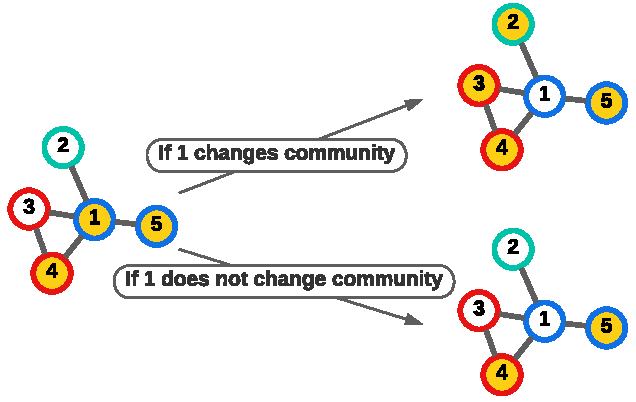
\includegraphics[width=0.78\linewidth]{out/rak-pruning.pdf}
  } \\[-2ex]
  \caption{Illustration of vertex pruning optimization: After processing vertex $1$, it's unmarked. If vertex $1$ changes its community, its neighbors are marked for processing. Community membership of each vertex is depicted by border color, and marked vertices are highlighted in yellow \cite{sahu2023gvelouvain}.}
  \label{fig:rak-pruning}
\end{figure}



\subsubsection{Picking the best label}

When there exist multiple labels connected to a vertex with maximum weight, we may randomly pick one of them (non-strict LPA), or pick only the first of them (strict LPA). We implement non-strict LPA using a simple modulo operator on the label id, as we observe that using \textit{xorshift} based random number generator does not provide any advantage. Results indicate that the strict version of LPA is $1.5\times$ faster than the non-strict approach, while also offering a gain in modularity of $2.1\%$.


\subsubsection{Hashtable design}

One can utilize C++'s inbuilt map as per-thread (independent) hashtables for the LPA algorithm. However, this exhibits poor performance. Therefore, we employ a key-list and a collision-free full-size values array to dramatically improve performance. However, if the memory addresses of the hashtables are nearby (\textit{Close-KV}), even if each thread uses its own hashtable exclusively, the performance is not as high. This is possibly due to false cache-sharing. Alternatively, if we ensure that the memory address of each hashtable is farther away (\textit{Far-KV}), the performance improves. Our results indicate that \textit{Far-KV} has the best performance and is $15.8\times$ times faster than \textit{Map}, and $2.6\times$ times faster than \textit{Close-KV} with LPA. An illustration of \textit{Far-KV} hashtable is in Figure \ref{fig:rak-hashtable}.

\begin{figure}[hbtp]
  \centering
  \subfigure{
    \label{fig:rak-hashtable--all}
    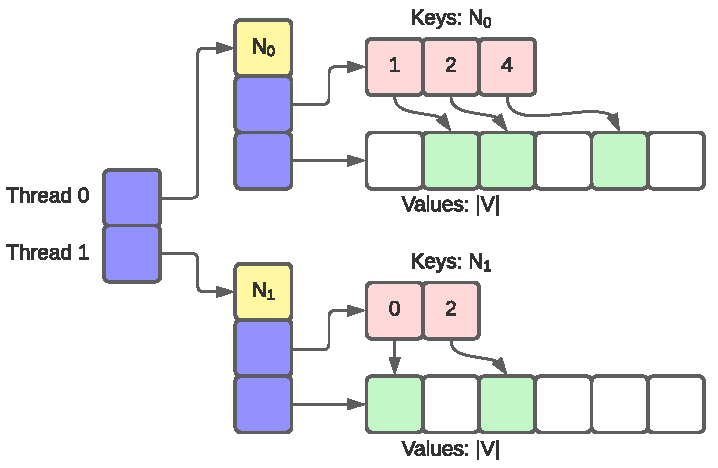
\includegraphics[width=0.88\linewidth]{out/rak-hashtable.pdf}
  } \\[-2ex]
  \caption{Illustration of collision-free per-thread hashtables that are well separated in their memory addresses (Far-KV), for two threads. Each hashtable consists of a keys vector, values vector (of size $|V|$), and a key count ($N_0$/$N_1$). The value associated with each key is stored/accumulated in the index pointed by the key. As the key count of each hashtable is updated independently, we allocate it separately on the heap to avoid false cache sharing \cite{sahu2023gvelouvain}.}
  \label{fig:rak-hashtable}
\end{figure}

\begin{figure*}[hbtp]
  \centering
  \subfigure{
    \label{fig:rak-opt--all}
    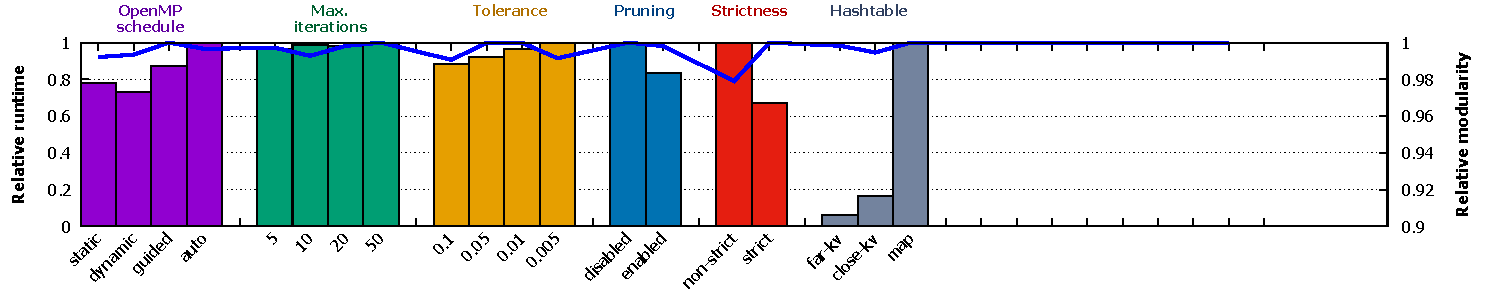
\includegraphics[width=0.98\linewidth]{out/rak-opt.pdf}
  } \\[-2ex]
  \caption{Impact of\ignore{various} parameter controls and optimizations on the runtime and result quality (modularity) of LPA. We show the impact of each optimization upon the relative runtime on the left Y-axis, and upon the relative modularity on the right Y-axis.}
  \label{fig:rak-opt}
\end{figure*}





\subsection{Our optimized LPA implementation}

We now explain the implementation of GVE-LPA in Algorithm \ref{alg:rak}. Its main step is the \texttt{lpa()} function (lines \ref{alg:rak--main-begin}-\ref{alg:rak--main-end}), which takes the input graph $G$ and assigns community memberships (or labels) $C$ to each vertex. In lines \ref{alg:rak--init-begin}-\ref{alg:rak--init-end}, we first initialize the labels $C$ of each vertex in $G$, and mark all vertices as unprocessed. We then perform iterations to propagate labels based on the weighted influence of neighboring vertices, limited to $MAX\_ITERATIONS$ (lines \ref{alg:rak--iters-begin}-\ref{alg:rak--iters-end}). In each iteration, we invoke the \texttt{lpaMove()} function to perform label propagation, and count the number of nodes with updated labels $\Delta N$ (line \ref{alg:rak--propagate}). If the ratio of $\Delta N$ to the total number of nodes $N$ is within a specified tolerance $\tau$, convergence has been achieved, and we terminate the loop (line \ref{alg:rak--converged}). Upon completing all iterations, we return the final labels $C$ (line \ref{alg:rak--main-return}).

\begin{algorithm}[hbtp]
\caption{GVE-LPA: Our parallel Label Propagation Algorithm (LPA).}
\label{alg:rak}
\begin{algorithmic}[1]
\Require{$G'$: Input graph}
\Require{$C$: Community membership of each vertex}
\Require{$G'$: Input/super-vertex graph}
\Require{$C'$: Community membership of each vertex in $G'$}
\Require{$K'$: Total edge weight of each vertex}
\Require{$\Sigma'$: Total edge weight of each community}
\Ensure{$G'_{C'}$: Community vertices (CSR)}
\Ensure{$H_t$: Collision-free per-thread hashtable}
\Ensure{$l_i$: Number of iterations performed (per pass)}
\Ensure{$l_p$: Number of passes performed}
\Ensure{$\tau$: Per iteration tolerance}
\Ensure{$\tau_{agg}$: Aggregation tolerance}

\Statex

\Function{louvain}{$G$} \label{alg:louvain--begin}
  \State Vertex membership: $C \gets [0 .. |V|)$ \textbf{;} $G' \gets G$ \label{alg:louvain--initialization}
  \ForAll{$l_p \in [0 .. \text{\small{MAX\_PASSES}})$} \label{alg:louvain--passes-begin}
    \State $\Sigma' \gets K' \gets vertexWeights(G')$ \textbf{;} $C' \gets [0 .. |V'|)$ \label{alg:louvain--reset-weights}
    \State Mark all vertices in $G'$ as unprocessed \label{alg:louvain--reset-affected}
    \State $l_i \gets louvainMove(G', C', K', \Sigma')$ \label{alg:louvain--local-move}
    \If{$l_i \le 1$} \textbf{break} \Comment{Globally converged?} \label{alg:louvain--globally-converged}
    \EndIf
    \State $|\Gamma|, |\Gamma_{old}| \gets$ Number of communities in $C$, $C'$
    \If{$|\Gamma|/|\Gamma_{old}| > \tau_{agg}$} \textbf{break} \Comment{Low shrink?} \label{alg:louvain--aggregation-tolerance}
    \EndIf
    \State $C' \gets$ Renumber communities in $C'$ \label{alg:louvain--renumber}
    \State $C \gets$ Lookup dendrogram using $C$ to $C'$ \label{alg:louvain--lookup}
    \State $G' \gets louvainAggregate(G', C')$ \label{alg:louvain--aggregate}
    \State $\tau \gets \tau / \text{\small{TOLERANCE\_DROP}}$ \Comment{Threshold scaling} \label{alg:louvain--threshold-scaling}
  \EndFor \label{alg:louvain--passes-end}
  \State $C \gets$ Lookup dendrogram using $C$ to $C'$ \label{alg:louvain--lookup-last}
  \Return{$C$} \label{alg:louvain--return}
\EndFunction \label{alg:louvain--end}
\end{algorithmic}
\end{algorithm}


The \texttt{lpaMove()} function (lines \ref{alg:rak--move-begin}-\ref{alg:rak--move-end}) iterates over unprocessed vertices in parallel. For each unprocessed vertex $i$ in the graph $G$, we mark $i$ as processed - vertex pruning (line \ref{alg:rak--prune}), obtain the total edge weight of connected labels in per-thread hashtable $H_t$ with the \texttt{scanCommunities()} function \ref{alg:rak--scan}, and select the most weighted label $c^*$ (line \ref{alg:rak--best-community}). If $c^*$ is not the same as the current label of $i$, we update the label of $i$, increment the count of changed vertices $\Delta N$, and mark the neighbors of $i$ as unprocessed for the next iteration (lines \ref{alg:rak--perform-move}-\ref{alg:rak--remark}). After having processed all vertices, we return the total number of vertices with updated labels $\Delta N$ (line \ref{alg:rak--move-return}). The \texttt{scanCommunities()} (lines \ref{alg:rak--scan-begin}-\ref{alg:rak--scan-end}) iterates over the neighbors of the current vertex $i$, excluding itself, and calculates the total weight of each label in the hashtable $H_t$.
